\section{Find Gravitational Acceleration}

Having established the initial separation $r = 125$ and the star's mass $M = 1000$, the initial gravitational acceleration of the planet can be computed. Recall from the Formulae section:

\begin{equation}
\vec{a} = -\frac{GM}{|\vec{r}|^3}\,\vec{r}
\end{equation}

where $\vec{r} = \vec{r}_p - \vec{r}_\star$ is the displacement vector from the star to the planet.

\subsection{Step-by-Step Calculation}

\textbf{Step 1.} Identify the displacement vector:
\begin{equation}
\vec{r} = \vec{r}_p - \vec{r}_\star = (100 - 0)\,\hat{\mathbf{i}} + (75 - 0)\,\hat{\mathbf{j}} = 100\,\hat{\mathbf{i}} + 75\,\hat{\mathbf{j}}
\end{equation}

\textbf{Step 2.} Compute $|\vec{r}|^3$ using the previously found distance $r = 125$:
\begin{equation}
|\vec{r}|^3 = 125^3 = 1{,}953{,}125 \approx 1.95 \times 10^6
\end{equation}

\textbf{Step 3.} Evaluate the scalar gravitational component:
\begin{equation}
-\frac{GM}{|\vec{r}|^3} = -\frac{1 \times 1000}{1{,}953{,}125} \approx -5.12 \times 10^{-4}
\end{equation}

\textbf{Step 4.} Multiply by the displacement vector:
\begin{align}
\vec{a} &= -5.12 \times 10^{-4} \times (100\,\hat{\mathbf{i}} + 75\,\hat{\mathbf{j}}) \\
        &\approx -0.0512\,\hat{\mathbf{i}} - 0.0384\,\hat{\mathbf{j}}
\end{align}

\textbf{Step 5.} Rounding to two decimal places:
\begin{equation}
\vec{a} \approx -0.05\,\hat{\mathbf{i}} - 0.04\,\hat{\mathbf{j}}
\end{equation}

\subsection{Physical Interpretation}

Both components of the acceleration are negative, meaning the planet is being pulled toward the third quadrant of the Cartesian plane — that is, directly toward the star which sits at the origin. This is precisely what we expect from an attractive gravitational force: the acceleration vector always points from the planet toward the star.

Figure~\ref{fig:cartesian} illustrates this geometrically. The planet in the first quadrant at $(100, 75)$ experiences a force directed toward the origin along the radial line connecting the two bodies.

\begin{figure}[H]
\centering
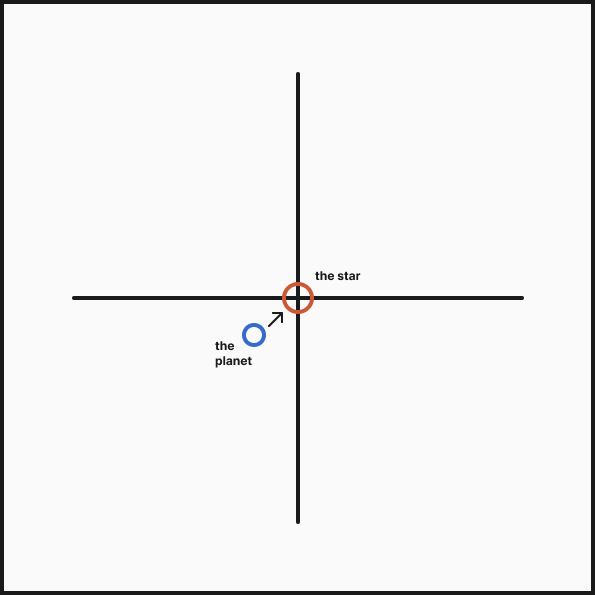
\includegraphics[width=0.5\textwidth]{figures/square.png}
\caption{Cartesian plane showing the planet's initial position and the direction of its gravitational acceleration, pointing back toward the star at the origin.}
\label{fig:cartesian}
\end{figure}

It is worth noting that the magnitude of the initial acceleration is relatively small ($|\vec{a}| \approx 0.064$). This is consistent with the planet being at a substantial distance from the star — gravitational force falls off as $1/r^2$, so larger separations yield weaker accelerations. The integration over many timesteps is what allows this small per-step force to curve the planet's path into a closed orbit.